%%% Template for documenting projects which involve circuit illustrations and code.
% Author: Claudiu Groza

% Template based on the template created by:
% Author:   Luis José Salazar-Serrano
%           totesalaz@gmail.com / luis-jose.salazar@icfo.es
%           http://opensourcelab.salazarserrano.com


\documentclass[a4paper,11pt]{article}

\usepackage[T1]{fontenc}
\usepackage[utf8]{inputenc}
\usepackage{graphicx}
\usepackage{xcolor}

\renewcommand\familydefault{\sfdefault}
\usepackage{tgheros}
\usepackage[defaultmono]{droidmono}

\usepackage{amsmath,amssymb,amsthm,textcomp}
\usepackage{enumerate}
\usepackage{multicol}
\usepackage{tikz}
\usepackage{courier}

\usepackage{pythonhighlight}

\usepackage{hyperref}

\usepackage{geometry}
\geometry{total={210mm,297mm},
left=25mm,right=25mm,%
bindingoffset=0mm, top=20mm,bottom=20mm}


\linespread{1.3}

\newcommand{\divider}{\rule{\linewidth}{0.5pt}}

% my own titles
\makeatletter
\renewcommand{\maketitle}{
\begin{center}
\vspace{2ex}
{\huge \textsc{\@title}}
\vspace{1ex}
\\
\divider\\
\@author \hfill \@date
\vspace{4ex}
\end{center}
}
\makeatother
%%%

% custom footers and headers
\usepackage{fancyhdr}
\pagestyle{fancy}
\lhead{}
\chead{}
\rhead{}
\lfoot{Alexa Pi Emulator}
\cfoot{}
\rfoot{Page \thepage}
\renewcommand{\headrulewidth}{0pt}
\renewcommand{\footrulewidth}{0pt}
%

% code listing settings
\usepackage{listings}

\lstset{%
  language = Octave,
  backgroundcolor=\color{white},   
  basicstyle=\footnotesize\ttfamily,       
  breakatwhitespace=false,         
  breaklines=true,                 
  captionpos=b,                   
  commentstyle=\color{gray},    
  deletekeywords={...},           
  escapeinside={\%*}{*)},          
  extendedchars=true,              
  frame=single,                    
  keepspaces=true,                 
  keywordstyle=\color{orange},       
  morekeywords={*,...},            
  numbers=left,                    
  numbersep=5pt,                   
  numberstyle=\footnotesize\color{gray}, 
  rulecolor=\color{black},         
  rulesepcolor=\color{blue},
  showspaces=false,                
  showstringspaces=false,          
  showtabs=false,                  
  stepnumber=2,                    
  stringstyle=\color{orange},    
  tabsize=2,                       
  title=\lstname,
  emphstyle=\bfseries\color{blue}%  style for emph={} 
} 

%%%----------%%%----------%%%----------%%%----------%%%

\begin{document}

\title{Alexa Pi Emulator}

\author{Anca Ilienescu, Remus Jeberean, Politehnica University of Timisoara}

\date{May, 2018}

\maketitle

\section{Repository}
\textbf{\url{https://github.com/ankies07/AlexaPi}}

\section{User requirements}

\begin{enumerate}  
\item Easy setup/installation process.
\item Wake-up word "Alexa".
\item Basic Alexa functionalities.
\item Open for extension eg. adding user-specific functionalities. 
\item LED notification indicating the state of the system.
\end{enumerate}

\section{System overview}
%\textit{Illustrate how you engineered the system from a generic point of view. You should point out all the important subsystems, modules or entities.}\\

The overview of the system is depicted in Figure \ref{fig:system}.

 \begin{figure}[h]
 \centering
  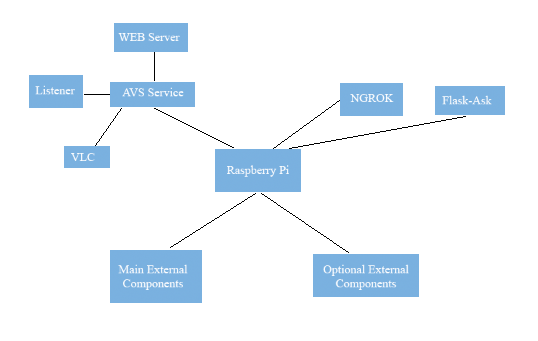
\includegraphics[scale=0.5]{PIC1.png}
 \caption{System overview diagram}
  \label{fig:system}
 \end{figure}

The entire system runs on the Raspberry Pi.\\

The required external components are comprised of a pair of speakers and a microphone. \\

Extensions to the system come under the form of Alexa's Skills. Skills are for Alexa what apps are for iOS or Android devices.\\

The system runs automatically on startup and requires no further input from the user outside of the first-time setup.\\

The microphone listens for the wake word "Alexa" and sends the voice input over the Cloud to the Amazon servers, where it is processed. A response is then received and played to the user through the speakers.\\

The AVS Service runs on startup and handles all Alexa related requests. It uses a small web server to generate the authentication tokens. It also uses a local listener (Pocketsphinx, an open-source engine) to listen for the word “Alexa” in order to start sending requests to the Alexa Voice Service. Responses are played back using VLC media player.\\

NGROK is a command-line program that opens a secure tunnel to localhost and exposes that tunnel behind an HTTPS endpoint, allowing Alexa to talk to the code on the Pi right away. \\

Flask-Ask is a Flask extension that helps building Alexa skills, making requests and responses easy to manage. The code using Flask-Ask will run on a while True loop, waiting for requests from the defined Intents received through NGROK. This code runs locally, on the Pi, not on the Amazon servers.
This means that any action triggered by Alexa voice commands happens on the Pi, and not on the Amazon servers, allowing for more functional and personal scripts to be run.\\

Main external components are the two LEDs and the button we may use for this system itself, while the optional ones represent anything else connected to GPIO.\\



\section{Circuit design}

The hardware view of the system is depicted below.

\begin{figure}[h]
\centering
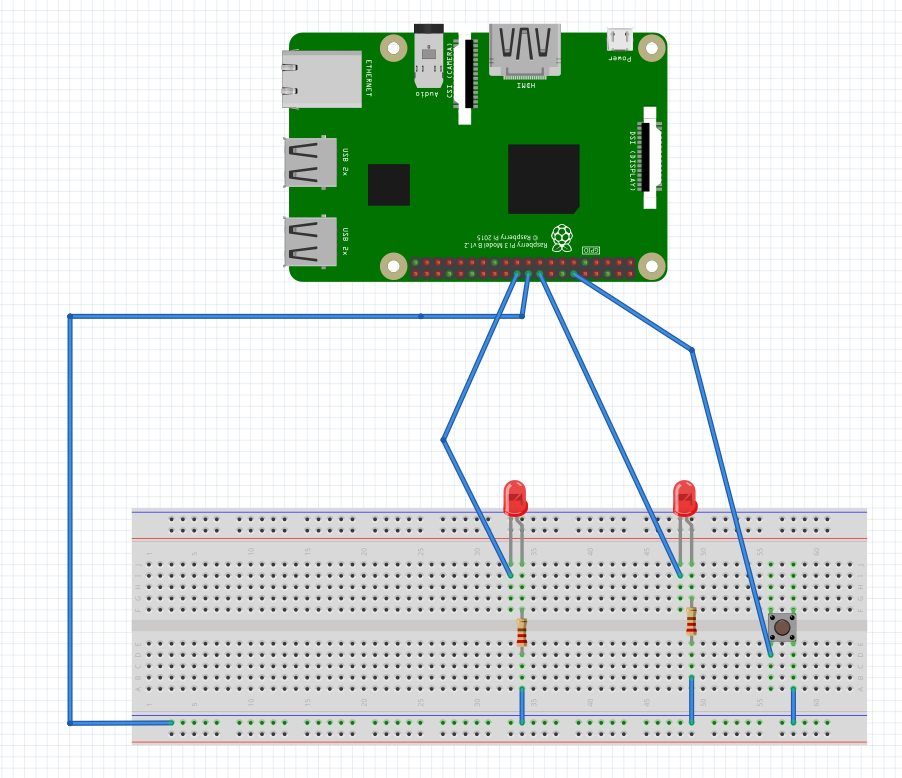
\includegraphics[scale=0.7]{PIC2.png}
\caption{Circuit schematic}
\label{fig:circuit-design}
\end{figure}

The Raspbery Pi 3 comes with everything we need on a fresh Raspbian install.\\

The only hardware components further required are speakers and a microphone. Any can be used, as long as they can connect to the Pi. This is most easily done with a USB to 3.5 jack adapter.\\

The wiring between the components can be seen in the figure above. It is important to note that, unless changed in the config file, the LEDs must be connected to GPIO 24 and 25, and the button to 18.\\

\section{Software design}

The software components and data flow directions are depicted in Figure \ref{fig:soft-design}. Each of these will be presented in the following subsections.\\

\begin{figure}
\centering
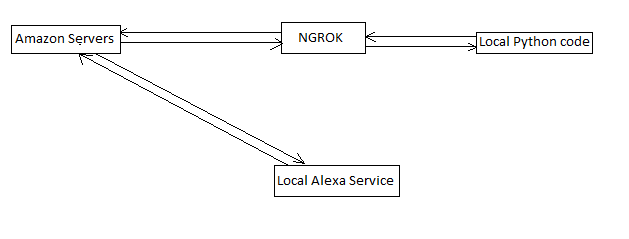
\includegraphics[scale=0.7]{PIC3.png}
\caption{Software entities involved}
\label{fig:soft-design}
\end{figure}
 
\subsection{Python modules} 
auth\_web.py: simple web server to generate authentication token using OAuth\\
main.py: main client, runs on a while True loop waiting for the triggered word “Alexa”. Once activated, records audio, sends it to the Amazon servers for processing and plays the response through VLC\\
\_\_function\_\_.py: local python scripts that may be activated using voice commands. These run using Flask-Ask and communicate with Alexa using NGROK. \\



\section{Results and further work}


The current version of the project supports the following functionalities:
\begin{itemize}  
\item Basic Alexa Integration: every command supported by default on Alexa enabled devices
\item Automatic Initialization on Setup
\item Running custom functions defined by the user
\item Configurable with respect to input/output device\\
\end{itemize}

The following list of extensions and improvements was identified to be supported in the future:
\begin{itemize}  
\item Using lambda functions for Alexa, eliminating the need for GROK and Flask-Ask
\item New functionality through new scripts
\end{itemize}



\end{document}